\chapter{Resultados}

Na tabela \ref{tabela} são apresentados os resultados obtidos para o algoritmo de \textit{smoothing}. Foram feitos testes para valores de N até 80000 sendo feita uma descrição detalhada do tempo para cada secção do programa desenvolvido. Nas tabelas \ref{tabela1} e \ref{tabela2} é feita uma previsão dos tempos quer para o CPU quer para o GPU (previsão feita com base nas linhas de tendência dos valores até 80000).

\begin{figure}[H]
	\begin{center}
		\makebox[\textwidth][c]{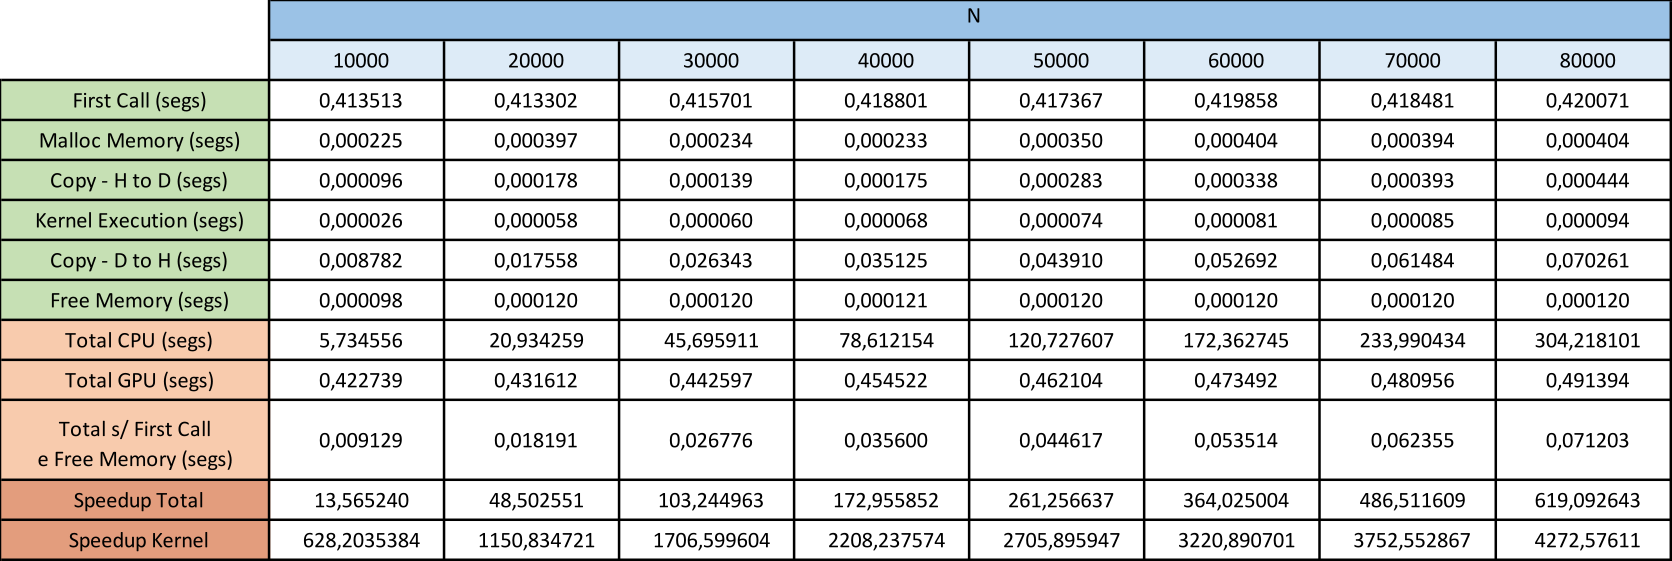
\includegraphics[clip, keepaspectratio=true, scale=3.5]{tabela.png}}
		\caption{Resultados Obtidos.}
		\label{tabela}
	\end{center}
\end{figure}

\begin{figure}[H]
	\begin{center}
		\makebox[\textwidth][c]{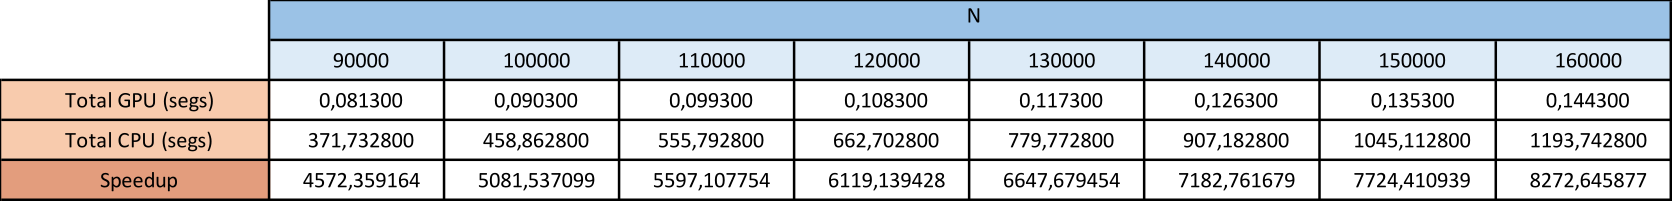
\includegraphics[clip, keepaspectratio=true, scale=3.5]{tabela1.png}}
		\caption{Previsão de Resultados.}
		\label{tabela1}
	\end{center}
\end{figure}

\begin{figure}[H]
	\begin{center}
		\makebox[\textwidth][c]{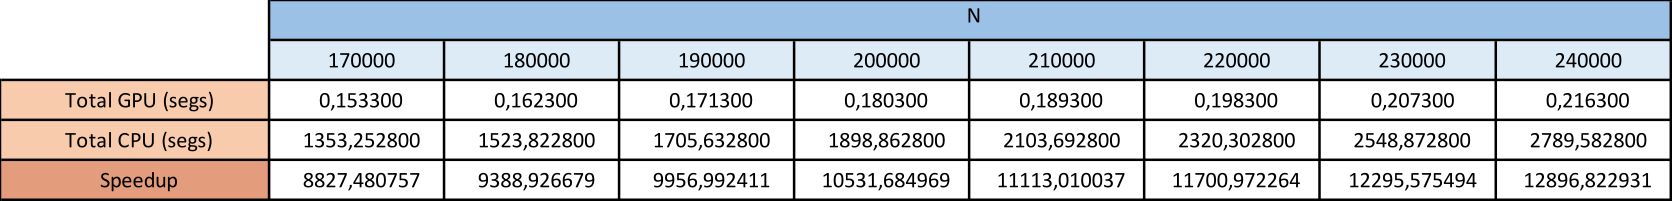
\includegraphics[clip, keepaspectratio=true, scale=3.5]{tabela2.png}}
		\caption{Previsão de Resultados (continuação).}
		\label{tabela2}
	\end{center}
\end{figure}

Com os valores obtidos através de baterias de 30 execuções para cada N foram elaborados os gráficos com o tempo de execução do CPU, do GPU, do Kernel e por fim da relação N - Speedup.

\begin{figure}[H]
	\begin{center}
		\makebox[\textwidth][c]{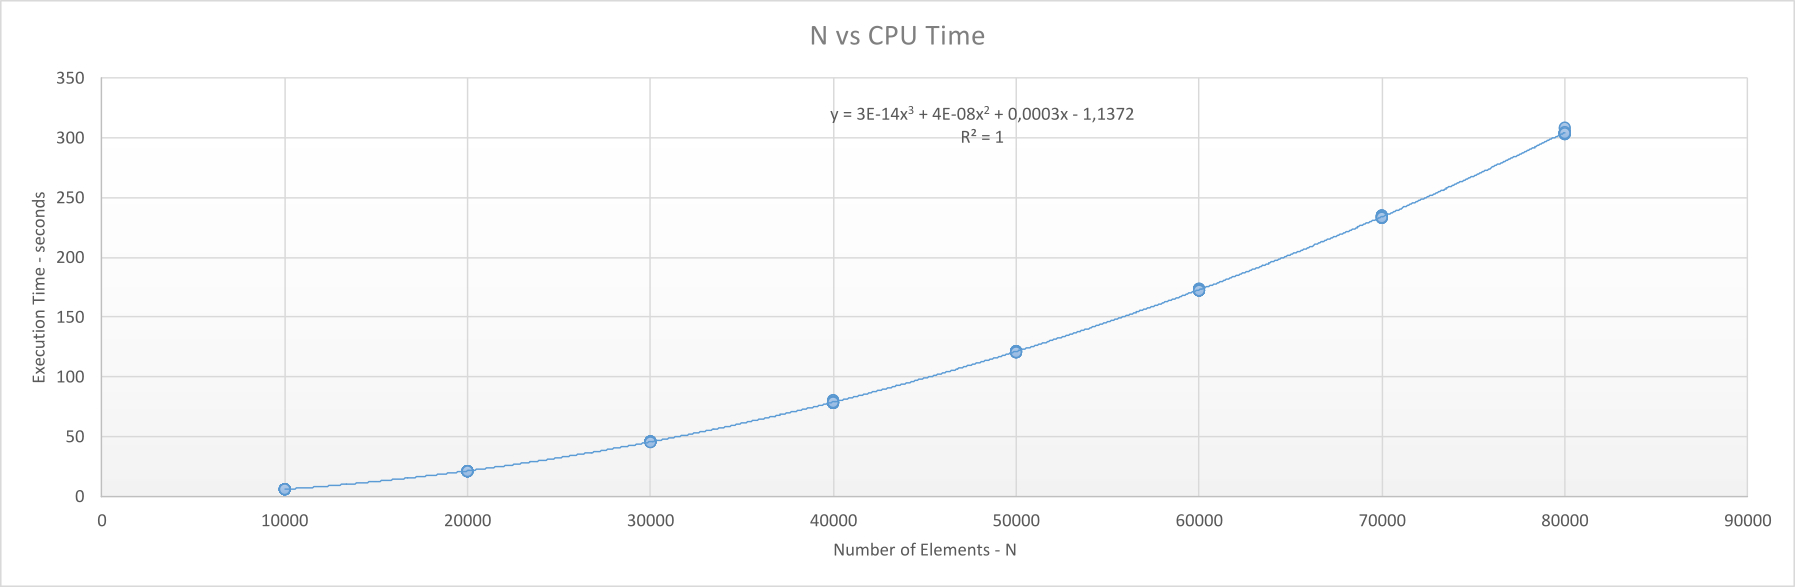
\includegraphics[clip, keepaspectratio=true, scale=2.5]{cpu.png}}
		\caption{Relação N - Tempo de CPU.}
		\label{cpu}
	\end{center}
\end{figure}

\begin{figure}[H]
	\begin{center}
		\makebox[\textwidth][c]{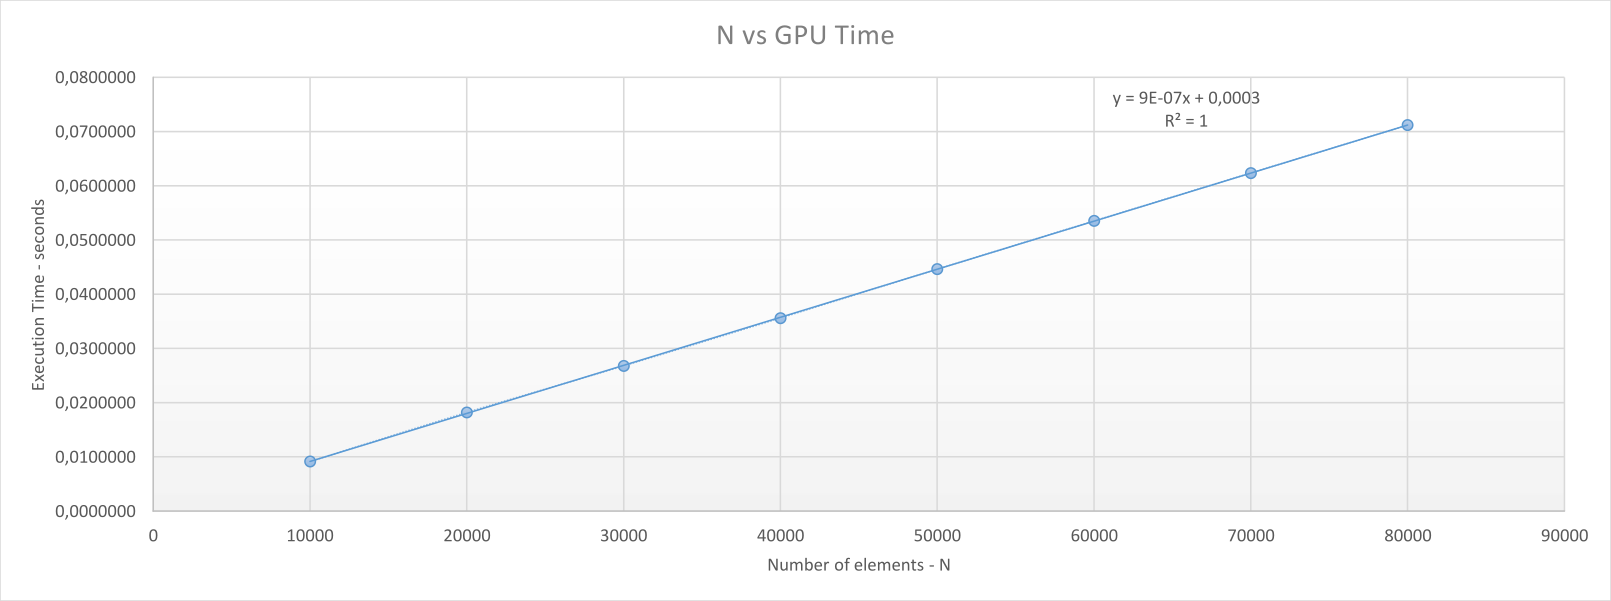
\includegraphics[clip, keepaspectratio=true, scale=2.5]{gpu.png}}
		\caption{Relação N - Tempo de GPU.}
		\label{gpu}
	\end{center}
\end{figure}

\begin{figure}[H]
	\begin{center}
		\makebox[\textwidth][c]{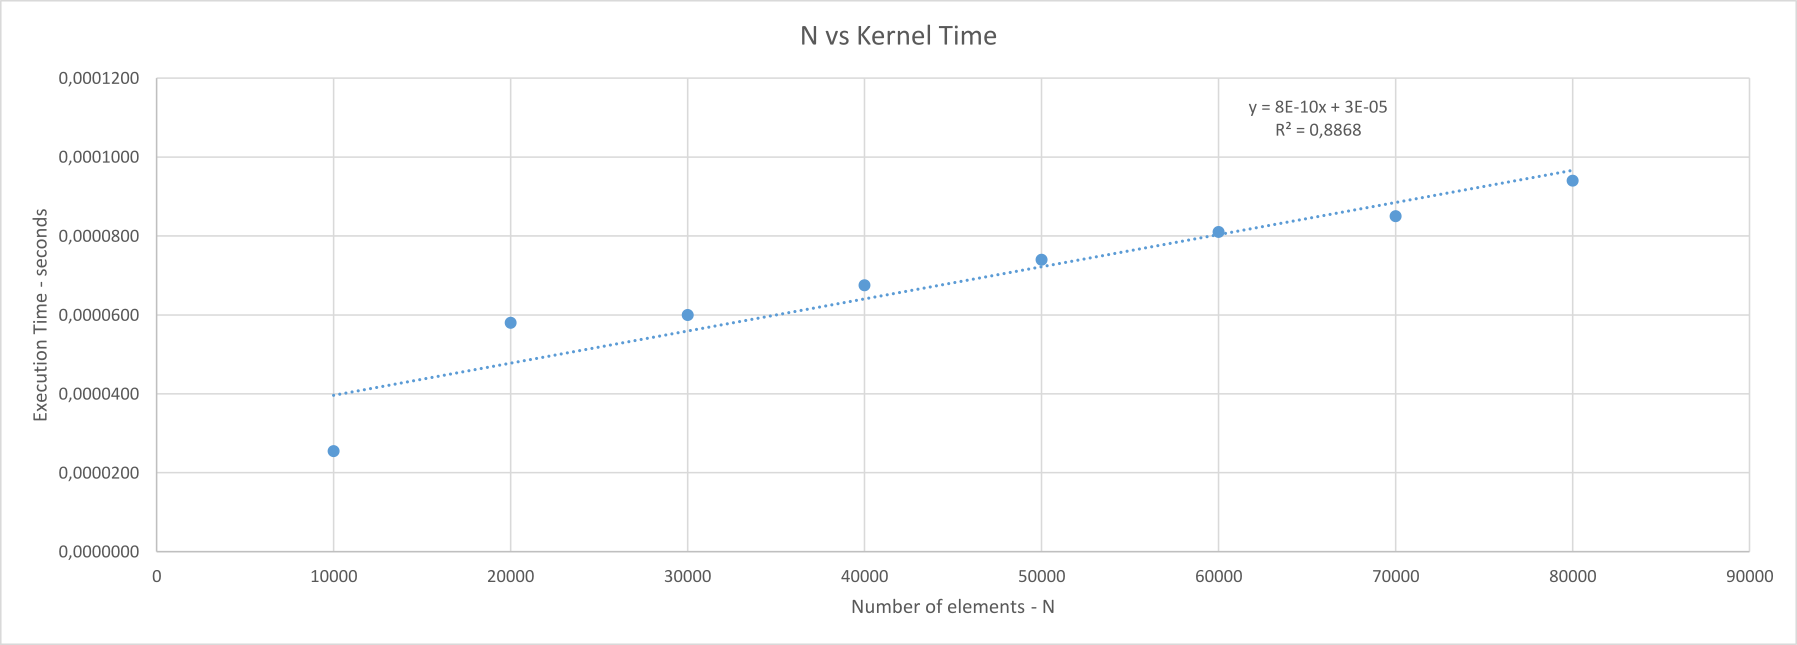
\includegraphics[clip, keepaspectratio=true, scale=2.5]{kernel.png}}
		\caption{Relação N - Tempo de Kernel.}
		\label{kernel}
	\end{center}
\end{figure}

\begin{figure}[H]
	\begin{center}
		\makebox[\textwidth][c]{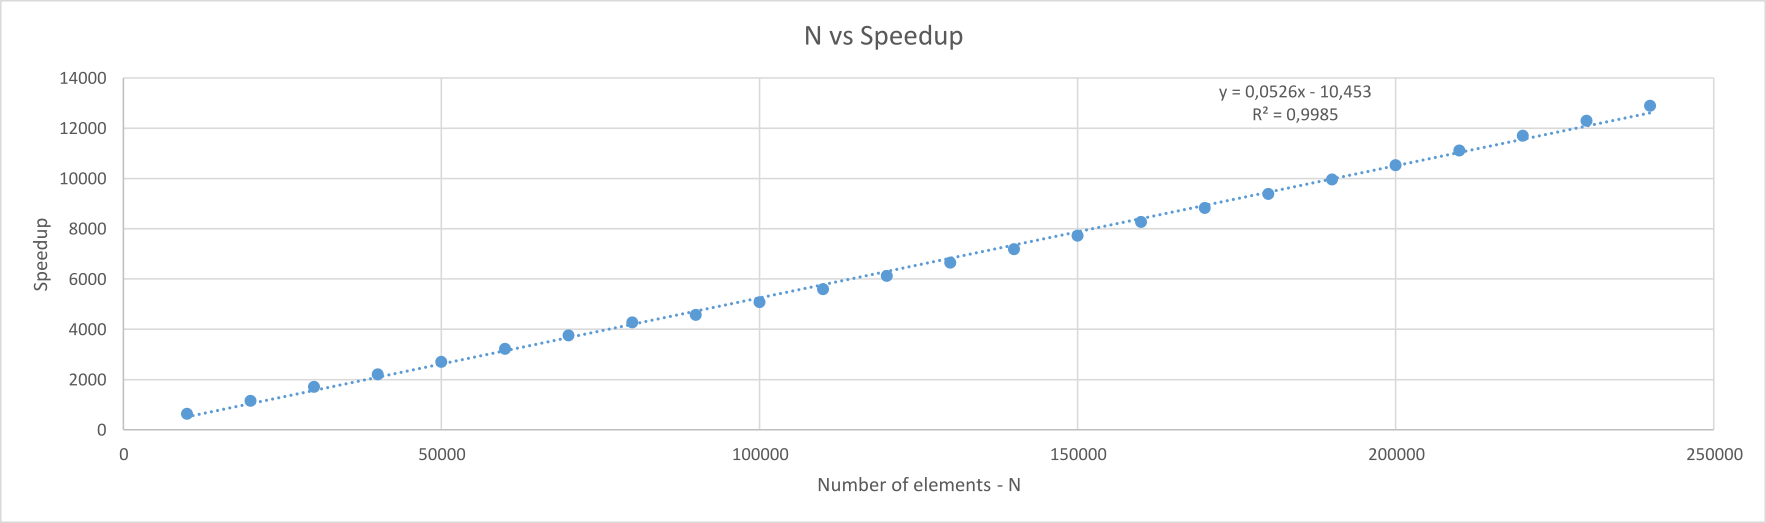
\includegraphics[clip, keepaspectratio=true, scale=2.5]{speedup.png}}
		\caption{Relação N - Speedup.}
		\label{speedup}
	\end{center}
\end{figure}

Por observação dos gráficos \ref{cpu} e \ref{gpu} é óbvio a utilização de \textit{GPUs} para este tipo de algoritmo. No caso do \textit{CPU} para N elevados o tempo de execução começa-se a obter uma função do tipo exponencial ao contrário do \textit{GPU} que mantêm um comportamento linear com crescimento imposto pelo tempo de tranferência de dados do \textit{Device} para o \textit{Host}.

Apesar de não serem apresentados valores de tempo para N inferior a 10000, tal como verificado na demonstração do programa na aula, o \textit{GPU} apresenta valores de Speedup inferior a 0.3 para N igual a 1000 e desta forma para valores de N baixos não se justifica a utilização de \textit{GPU} para este tipo de algoritmo. 
